\documentclass[11pt]{article}

\usepackage[margin=1in]{geometry}
\usepackage{booktabs}
\usepackage{graphicx}
\usepackage{microtype}
\usepackage{amsmath}
\usepackage{enumitem}
\usepackage{xcolor}
\usepackage{tikz}
\usetikzlibrary{arrows.meta,positioning}
\usepackage{pgfplots}
\pgfplotsset{compat=1.18}
\usepackage[numbers,sort&compress]{natbib}
\PassOptionsToPackage{hyphens}{url}
\usepackage[hidelinks]{hyperref}
\hypersetup{pdftitle={MeTTa-Scaffolded Repair Curricula for TRM-Infused Hermes Skills}, pdfauthor={Patrick Dugan}}

\newcommand{\pending}[1]{\textcolor{red}{[#1]}}
\newcommand{\testGoneq}{29 against 2 discordant, Holm $p < 0.001$}
\newcommand{\testGtwoq}{14 against 3 discordant, Holm $p = 0.013$}
\newcommand{\testGthreeq}{62 against 0 discordant, Holm $p < 0.001$}
\newcommand{\testGfourq}{57 against 0 discordant, Holm $p < 0.001$}
\newcommand{\testRoneq}{0 against 15 discordant, Holm $p < 0.001$}
\newcommand{\testRtwoq}{1 against 1 discordant, Holm $p = 1.00$}
\newcommand{\testMoneq}{12 against 1 discordant, Holm $p = 0.010$}
\newcommand{\testMtwoq}{2 against 3 discordant, Holm $p = 1.00$}
\newcommand{\testMthreeq}{3 against 0 discordant, Holm $p = 0.50$}
\newcommand{\testGone}{17 against 9 discordant, Holm $p = 0.34$}
\newcommand{\testGtwo}{16 against 16 discordant, Holm $p = 1.00$}
\newcommand{\testGthree}{59 against 0 discordant, Holm $p < 0.001$}
\newcommand{\testGfour}{51 against 1 discordant, Holm $p < 0.001$}
\newcommand{\testRone}{0 against 0 discordant, Holm $p = 1.00$}
\newcommand{\testRtwo}{4 against 0 discordant, Holm $p = 0.25$}
\newcommand{\testMone}{4 against 1 discordant, Holm $p = 0.75$}
\newcommand{\testMtwo}{6 against 0 discordant, Holm $p = 0.094$}
\newcommand{\testMthree}{0 against 0 discordant, Holm $p = 1.00$}
\newcommand{\testPone}{20 against 15 discordant, Holm $p = 1.00$}
\newcommand{\testPtwo}{18 against 8 discordant, Holm $p = 0.23$}
\newcommand{\testPthree}{30 against 0 discordant, Holm $p < 0.001$}
\newcommand{\testPfour}{11 against 8 discordant, Holm $p = 1.00$}
\newcommand{\testPfive}{37 against 6 discordant, Holm $p < 0.001$}
\newcommand{\testPsix}{32 against 9 discordant, Holm $p < 0.001$}
\newcommand{\testCone}{atoms 55--78 against raw 50--58 of 141, exact permutation Holm $p = 0.024$}
\newcommand{\testCtwo}{atoms 59--79 against raw 54--60 of 141, exact permutation Holm $p = 0.024$}

\setlength{\emergencystretch}{2em}

\title{MeTTa-Scaffolded Repair Curricula for TRM-Infused Hermes Skills}
\author{Patrick Dugan\\Morality Lab}
\date{April 29, 2026; revised October 2026}

\begin{document}
\maketitle

\begin{abstract}
We study MeTTa-scaffolded near-miss repair curricula for Hermes agent skills: a declared, typed account of a skill's verifier state that turns semi-failed outputs into training rows for tiny recursive models (TRMs) and other gates. The April version of this report proposed the method without training a TRM, on a curriculum whose rows carried no candidate content, and its rudder benchmark had two defects: a retrieval arm that selected examples using the hidden label, and an unseen-family split no model could answer. This revision re-obtains the April model, Qwen2.5-3B-Instruct, replicates the April runs with the April code, corrects both defects, and runs the missing experiment. The replication reproduces the April numbers within a few rows on every arm except the leaky retrieval arm, whose repair choice sits on near-tied tokens. On a Campsite logic-grid curriculum built from 1{,}312 real answers by Qwen2.5-3B, repairing and then asking the public verifier solves every answer the skill's operators can fix (63 of 148 test answers) and commits nothing broken. A tiny recursive gate trained before repair on the same rows solves 48 and commits 24 broken grids, and standard classifiers do no better: what the repair will do is not visible before it runs. Declaring the verifier atoms makes the gate learn from fewer rows and solve more than one trained on raw cells (48 against 37), and a gate trained on synthetic defects instead of real failures solves 21 and commits 66 broken grids. Two 1-bit models, Bonsai-8B and Bonsai-27B, show the same gate pattern with weaker effects. A TRM that writes the repair itself does better than the skill's operators: placed after them, it lifts the skill from 63 to 93 solved answers with no broken commit, with similar gains on the Bonsai models' answers. Framing its training corpus with cell atoms declared in a MeTTa package makes it three to four times as data-efficient: with a quarter of the corpus it solves 57 answers against 26. With the full corpus the two framings do not separate as five-model ensembles. Single framed models still solve about nine to ten more answers than single raw ones, which a fresh test pool with new seeds confirmed. On the output-contract suites, showing the 3B the validator's contract lifts it from 24 to 35 of 50, and the MeTTa gate wording adds nothing. The method survives with its roles made precise: declare the gates, let tables choose operators, let the verifier own the commit, train gates only on real failures, and train a repair TRM on a MeTTa-framed corpus where the operators stop.
\end{abstract}

\section{Motivation}

Hierarchical and recursive reasoning models have reopened the question of whether compact specialized models can do useful reasoning work without a very large language model at every step. HRM proposes a two-timescale recurrent architecture with strong sample efficiency on puzzle-like tasks \citep{wang2025hrm}; TRM simplifies this into a small recursive network with strong ARC-style results \citep{jolicoeurmartineau2025trm}. In parallel, MeTTa and OpenCog Hyperon provide a reflective metagraph language for representing rules, programs, and cognitive procedures as rewriteable symbolic objects \citep{goertzel2021metta,meredith2023metametta}.

Our setting combines these threads with instruction-tuned tool-use models in the Hermes line \citep{teknium2024hermes3} and with verifier environments of the kind released with INTELLECT-3 \citep{primeintellect2025intellect3}. The research question is narrow: can MeTTa-scaffolded symbolic state make tiny recursive gates trainable, from few rows, for the parts of an agent skill that decide what to repair and what to commit?

The question matters beyond benchmarks. If useful behavior can be compressed into small local models, recursive modules, symbolic validators, and skill-specific control graphs, then the security and power balance of AI will not be set only by who controls the largest training runs; it will also depend on how quickly capable behaviors can be distilled, routed, evaluated, and recombined into deployable hybrid systems. Adjacent work approaches this from other directions. COSPLAY co-evolves an LLM decision agent with a learnable skill bank extracted from rollouts \citep{wu2026cosplay}. Sakana's Fugu learns a small coordinator that routes work across pools of stronger models \citep{sakana2026fugu}. We study a third path: restructuring the skill itself so that symbolic gates, tiny trained gates, and a small language model carry the capability together.

The design rests on a pattern with a longer history. LLM-Modulo frameworks place a language model as a generator inside a loop whose external verifiers hold the authority to accept \citep{kambhampati2024llmmodulo}; AlphaGeometry pairs a language model that proposes constructions with a symbolic engine that closes the proof \citep{trinh2024alphageometry}; learned verifiers and process reward models judge candidates at large scale \citep{cobbe2021verifiers,lightman2024verify}. Studies of self-repair and self-correction find little gain when a model judges its own output without external feedback, and real gains when the feedback comes from a stronger source \citep{olausson2024selfrepair,huang2024selfcorrect}. Our skills follow that lesson: the commit decision belongs to a verifier wherever one exists, and the question is what is left for trained gates and for the model.

\section{Terms and prior baseline}
\label{sec:baseline}

\paragraph{Two meanings of TRM.} Earlier Hermes Skills work used ``TRM'' for a \emph{task-representation memory}: a bank of replayed rows (critic labels, exact positives, negatives) consulted by retrieval. This paper uses TRM for a \emph{tiny recursive model}: a small network that applies one update step several times to a latent state, following \citet{jolicoeurmartineau2025trm}. The gates trained in Section~\ref{sec:training} use the structure of hermes-lite's \texttt{TinyRecursivePolicy}: an input projection, a recurrent update on the concatenated input and state applied four times, and an action head, with a 64-unit state. The April version of this paper used both meanings without saying so.

\paragraph{The April 16--22 baseline.} That week's runs on PrimeHub-style environments with Qwen3.5-9B and Qwen3.5-27B left a task-representation memory of 195 rows (24 exact positives, 5 weak positives, 166 negatives). In its run ledger, critic bucket accuracy was 0.75 and retriever exact match was 0.0625. The memory was useful for criticism and abstention and too sparse to generate actions. Grouping its rows by role showed the same thing: answer-format roles (\texttt{choice\_contract}, \texttt{structured\_map}) held most of the action-bearing positives, while the hard-reasoning and abstain roles behaved as critics. We report these numbers as descriptive; they come from a single week's ledger and are not re-measured here.

\section{Method: near-miss repair curricula}
\label{sec:method}

A near-miss repair curriculum turns semi-failed outputs into training rows. Each row records the environment family, the candidate, the verifier's typed verdict, the outcome of each declared repair operator, a bucket, and the decision a gate should have made. One failed output is thereby usable as a verifier example, a repair example, a preservation example, or a hard negative for a commit gate.

\paragraph{The April curriculum.} The April curriculum has 244 rows from three sources: 218 from a replay of Campsite logic-grid repairs (the INTELLECT-3 logic environment), 20 from a deterministic proposal-tier suite, and 6 from small-model probes. Rows from the same base case stay in the same split, and six failure labels are reserved for an unseen-family holdout (Table~\ref{tab:splits}). Two properties limit what can be trained on it. The Campsite rows carry no candidate content: the candidate field reads \texttt{arm=logic\_skill\_trm transform=original}, so a model sees only labels. And two of the state fields, the candidate's reward and the distinction between an exact grid and a grid that passes the count checks but has a wrong cell, are computed against the answer key, which a deployed skill does not have.

\begin{table}[t]
  \centering
  \small
  \begin{tabular}{lrrrrr}
    \toprule
    Split & Rows & Exact positive & Repair success & Partial improvement & No gain \\
    \midrule
    Train & 156 & 46 & 58 & 12 & 40 \\
    Validation, seen family & 34 & 14 & 12 & 2 & 6 \\
    Holdout, seen family & 36 & 8 & 12 & 6 & 10 \\
    Holdout, unseen family & 18 & 3 & 9 & 0 & 6 \\
    \bottomrule
  \end{tabular}
  \caption{The April near-miss curriculum. The 222 Campsite rows are pairs: a count-only repair and a dual repair of the same grid. The 88 non-train rows cover 44 source problems.}
  \label{tab:splits}
\end{table}

\paragraph{A curriculum with content.} To train gates for real, this revision builds a Campsite curriculum whose rows carry the candidate grid. Puzzles come from hermes-lite's generator (3$\times$5 to 6$\times$6), split by puzzle hash into train (300), validation (58), and test (148). The verifier is hermes-lite's official checker, which reads only public rules: symbols, shape, trees unchanged, row and column tent counts, no touching tents, and a perfect tree--tent matching. The generator does not guarantee a unique solution, so success always means passing the verifier. The repair operators are the skill's own: \texttt{c\_repair}, a minimum-edit projection of the tents onto the row and column counts that keeps the candidate's trees, and \texttt{dual\_repair}, which also restores the row and column tree counts. Both read only public counts. Candidates come from two sources:
\begin{itemize}[leftmargin=*]
  \item \textbf{real near-misses}: local models answering each puzzle from a three-shot prompt on CPU. Qwen2.5-3B-Instruct at 4 bits (the April model) and Bonsai-8B, a 1-bit 8B model \citep{prismml2026bonsai}, give one greedy and two sampled answers per train puzzle and one greedy and one sampled per validation and test puzzle; Bonsai-27B answers each test puzzle once, greedily;
  \item \textbf{synthetic near-misses}: eight defect types applied to a known solution (dropped, extra, or moved tents; a swapped rectangle of tents; a mutated tree; a ragged row).
\end{itemize}
Each row's label is the first action in the menu (commit, \texttt{c\_repair}, \texttt{dual\_repair}) whose result passes the verifier, and reject if none does.

\section{The MeTTa layer}
\label{sec:metta}

The MeTTa contribution is a typed declaration layer above individual skills. A composition grammar wires skills into circuits while respecting roles: formatters do not become solvers, critics do not become action generators, and hard-reasoning roles stay verifiers until their positives justify more. A new skill fork is designed as
\[
\mathrm{observe} \rightarrow \mathrm{route} \rightarrow \mathrm{propose} \rightarrow \mathrm{validate} \rightarrow \mathrm{repair} \rightarrow \mathrm{validate} \rightarrow \mathrm{commit\ or\ veto} \rightarrow \mathrm{learn},
\]
and each gate emits a typed record, so evaluation data are produced by construction.

What the layer is, concretely: each skill family has a MeTTa package (one top-level atom per line) that a small compiler reads. For the Campsite curriculum, the package declares 16 feature atoms (the verifier's seven gates, seven distance-to-constraint counts, and the grid's dimensions), the two repair operators with their preconditions, the action menu, and the bucket rules. The compiler emits the feature schema: a row's typed state is exactly the declared atoms in declared order, and an atom the code does not compute is an error. No MeTTa interpreter runs at inference time. The tables and rules that the April version described as ``MeTTa owning'' a decision are Python functions implementing what a package declares. Whether MeTTa, as opposed to a well-organised JSON schema, adds anything is a question this paper does not test; what it tests is whether declaring the verifier-visible state changes what a tiny gate can learn.

\begin{figure}[t]
  \centering
  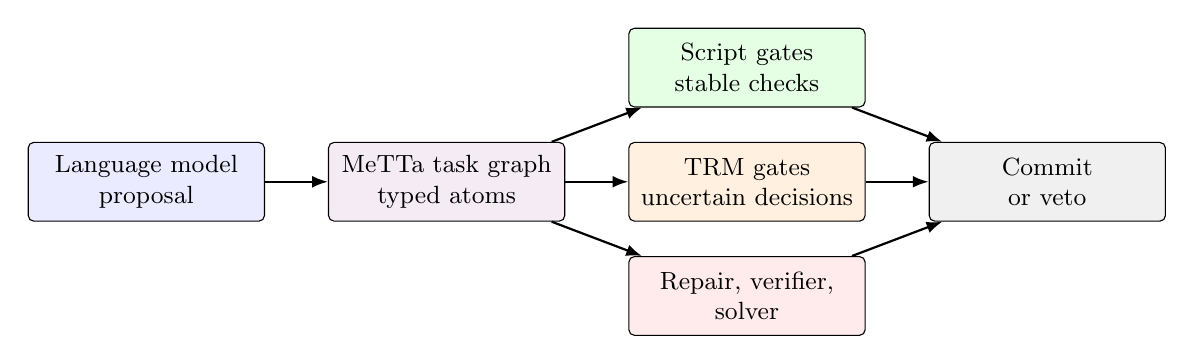
\begin{tikzpicture}[
      box/.style={draw, rounded corners=2pt, minimum width=3.0cm, minimum height=1.0cm, align=center, font=\small},
      arr/.style={-{Latex[length=2mm]}, thick}]
    \node[box, fill=blue!8] (llm) {Language model\\proposal};
    \node[box, fill=violet!8, right=0.8cm of llm] (graph) {MeTTa task graph\\typed atoms};
    \node[box, fill=green!10, right=0.8cm of graph, yshift=1.45cm] (script) {Script gates\\stable checks};
    \node[box, fill=orange!12, right=0.8cm of graph] (trm) {TRM gates\\uncertain decisions};
    \node[box, fill=red!8, right=0.8cm of graph, yshift=-1.45cm] (solver) {Repair, verifier,\\solver};
    \node[box, fill=gray!12, right=0.8cm of trm] (commit) {Commit\\or veto};
    \draw[arr] (llm) -- (graph);
    \draw[arr] (graph) -- (script);
    \draw[arr] (graph) -- (trm);
    \draw[arr] (graph) -- (solver);
    \draw[arr] (script) -- (commit);
    \draw[arr] (trm) -- (commit);
    \draw[arr] (solver) -- (commit);
  \end{tikzpicture}
  \caption{Task-graph allocation. The package names the gates; each gate goes to the cheapest executor that is reliable for it.}
  \label{fig:schema}
\end{figure}

\section{The rudder benchmark}
\label{sec:rudder}

\subsection{Setup}

Before training any gate, the April version asked whether a small language model could act as a ``rudder'' over the curriculum: from a row's typed state, choose the repair action and whether to commit. The benchmark uses the 88 non-train rows. The model sees the environment family, role, the arms before and after repair, the candidate's reward, the failure label, the uninformative candidate field, and two gate outputs; it never sees the bucket or the target. The published arms were \textbf{raw} (choose an action from the six that occur in training, and commit or reject), \textbf{retrieval} (raw plus four retrieved training rows with their answers), \textbf{action-space} (a table keyed on family and failure label fixes the repair action; the model only commits or rejects), and \textbf{static gate} (three rules on visible labels decide first: an exact label commits, a passed-counts-but-wrong-cell label rejects, an empty or weak proposal tier rejects; the model decides the rest). The April run used Qwen2.5-3B-Instruct at 4 bits (greedy, 64 tokens); a May run added Qwen3.5-9B and Qwen3.5-27B at 4 bits with thinking disabled.

\subsection{Two defects}

\paragraph{The retrieval arm used the answer.} The retriever scored training rows by token overlap with the query, and the query's tokens included its own bucket, repair action, and target action, with a bonus for a matching bucket. For each of the four rows whose repair produced no gain, all four retrieved examples were no-gain rows, against a base rate of 17 in 86. The 9B and 27B copied the majority label of their examples on all 36 count-repair rows.

\paragraph{The unseen-family actions were unreachable.} The 18 unseen-family rows need repair actions that do not occur in training and were therefore not in the list shown to the model. Every model-decided arm scores 0 of 18 on them by construction. The action-space table scores 18 of 18 because its authors wrote entries for those families.

\subsection{What the published arms measure}

\begin{table}[t]
  \centering
  \small
  \begin{tabular}{lrrrrrr}
    \toprule
    & \multicolumn{3}{c}{Joint, of 88} & \multicolumn{3}{c}{False commits, of 22} \\
    \cmidrule(lr){2-4} \cmidrule(lr){5-7}
    Published arm & \hspace{1.2em}3B & \hspace{1.2em}9B & 27B & \hspace{1.2em}3B & \hspace{1.2em}9B & 27B \\
    \midrule
    Raw & 32 & 32 & 43 & 22 & 18 & 21 \\
    Retrieval (leaks the label) & 28 & 70 & 70 & 18 & 0 & 0 \\
    Action-space & 66 & 66 & 71 & 22 & 22 & 16 \\
    Static gate & 84 & 84 & 83 & 4 & 4 & 4 \\
    \bottomrule
  \end{tabular}
  \caption{The published rudder arms, rescored from their row-level results. The 88 rows are 44 source problems.}
  \label{tab:rudder-pub}
\end{table}

Table~\ref{tab:rudder-pub}. Three readings follow from the rows. First, the action-space lift is a lookup: on this data the repair action is a function of the failure label, and fixing it adds 34 correct rows at 3B (34 against 0 discordant, $p<0.001$). Second, the model's share of the static-gate arm is a constant. The rules decide 43 rows from labels; of the 45 left, 41 should commit and 4 should reject, and the 3B and 9B commit all 45, which is exactly what a policy that always commits scores (the 27B commits 44). In the action-space arm the 3B and 9B commit all 88 rows. Third, scale moves only the raw arm, and only through the repair action: from 3B to 9B the raw arm is unchanged and right on the same 32 rows; the 27B gains 11, all on the repair action, while still committing 21 of 22 no-gain repairs. The four no-gain rows left to the model in the static-gate arm are two grids in both repair variants; nothing visible before repair separates them from the 32 count-repair rows that succeeded, and no model at any size vetoes them.

A May revision of the static rules added two rules that read the post-repair bucket, after which the arm scores 88 of 88 without a model call. Since the target is defined from that bucket, the revision restates the label and is not a result.

\subsection{Replication with the April model}

The April model was re-obtained for this revision: the file \texttt{qwen2.5-3b-instruct-q4\_k\_m.gguf} from the official Qwen repository, pinned to a revision and checked against its published SHA-256. The April 28 version of the benchmark runner, the last before the May rules, was executed unchanged from the repository on the same splits, with temperature 0, top-p 1, an 8-bit KV cache, and the April context and token caps. Two things differ: this revision runs on CPU with a different llama.cpp build, where April used a CUDA build, and it uses more threads and a larger batch for speed. Two arms are new: \emph{clean retrieval} scores examples on pre-repair fields only, and \emph{full vocabulary} lists all twelve repair actions so the unseen-family rows become reachable. Both use the April runner's own prompt builder and generation call (Table~\ref{tab:rudder-qwen}).

\begin{table}[t]
  \centering
  \small
  \resizebox{\linewidth}{!}{\begin{tabular}{lrrrrr}
\toprule
Arm & Joint, April & Joint, rerun & Same answers as April & False commits & Unseen-family joint \\
& of 88 & of 88 & rows & of 22 & of 18 \\
\midrule
Raw, six train actions & 32 & 32 & 84/88 & 22 & 0 \\
Raw, all twelve actions & -- & 1 & new arm & 12 & 0 \\
Retrieval, published (leaks the label) & 28 & 17 & 73/88 & 18 & 0 \\
Retrieval, pre-repair fields only & -- & 17 & new arm & 21 & 0 \\
Action-space & 66 & 66 & 88/88 & 22 & 12 \\
Action-space with retrieval & 61 & 60 & 85/88 & 22 & 7 \\
Static gate (April rules) & 84 & 84 & 88/88 & 4 & 18 \\
Post-repair oracle (no model) & 88 & 88 & 88/88 & 0 & 18 \\
\bottomrule
\end{tabular}
}
  \caption{The rudder benchmark with Qwen2.5-3B-Instruct, April run against this revision's CPU rerun of the April runner. ``Same answers'' counts rows whose repair action and commit decision both match the April row. ``Joint'' needs both decisions right.}
  \label{tab:rudder-qwen}
\end{table}

\begin{itemize}[leftmargin=*]
  \item \textbf{The April numbers replicate, except the leaky arm.} Raw, action-space, and static-gate arms reproduce the April joint scores exactly (32, 66, 84), with the same answer on 84, 88, and 88 of 88 rows. The leaky retrieval arm drops from 28 to 17: its retrieved examples are identical on all 88 rows, its commit decisions agree on every row, and all 15 disagreements are dual-repair rows where April chose \texttt{dual\_repair} and the rerun chose \texttt{c\_repair}. The arm's repair choice sits on near-tied tokens that flip between builds, so its April 28 is not a stable number.
  \item \textbf{Honest retrieval hurts the 3B.} With four clean examples in the prompt the 3B scores 17 against 32 raw (R1q: \testRoneq): it picks \texttt{c\_repair} on rows that need \texttt{dual\_repair}. Its commit decisions barely move (66 right against 65).
  \item \textbf{On this build the leak does not move the 3B.} Leaky and clean retrieval tie at 17 (R2q: \testRtwoq). The published retriever still hands the model examples whose label matches the hidden one 98.6\% of the time, against 77.3\% for the clean one; the 3B commits on 84 and 86 of 88 rows respectively.
  \item \textbf{Reachability exposes a format failure, not transfer.} With all twelve actions listed, the 3B copies the answer template \texttt{commit|reject\_or\_abstain} into its output on 60 of 88 rows and scores 1.
  \item \textbf{The action-space arm is a constant.} The 3B commits all 88 rows, as in April.
\end{itemize}

A second model gives the same picture (Table~\ref{tab:rudder-rerun}). Bonsai-8B, a 1-bit 8B, scores 32 raw and 32 with clean retrieval (R1: \testRone), where clean retrieval improves its commit decisions (false commits 9 against 22) but not its repair choice; the leaky retriever lifts it to 36 with a single false commit (R2: \testRtwo); with all actions listed it scores 17; its action-space arm also commits every row. Two arms need no language model at all: a two-head TRM on the published state fields and a lookup of the training majority per failure label both score 66, the action-space arm's score, and neither can produce an action it never saw.

\begin{table}[t]
  \centering
  \small
  \resizebox{\linewidth}{!}{\begin{tabular}{lrrrrrr}
\toprule
Arm & Joint & Repair & Commit/reject & Commits & False commits & Unseen-family joint \\
& of 88 & of 88 & of 88 & of 88 & of 22 & of 18 \\
\midrule
Raw, six train actions & 32 & 36 & 65 & 87 & 22 & 0 \\
Raw, all twelve actions & 17 & 19 & 66 & 88 & 22 & 1 \\
Retrieval, published (leaks the label) & 36 & 36 & 85 & 65 & 1 & 0 \\
Retrieval, pre-repair fields only & 32 & 36 & 78 & 74 & 9 & 0 \\
Action-space & 66 & 88 & 66 & 88 & 22 & 12 \\
Lookup, train majority (no model) & 66 & 70 & 78 & 76 & 10 & 0 \\
Two-head TRM, 4.3M parameters (no LLM) & 66 & 70 & 80 & 72 & 7 & 0 \\
\bottomrule
\end{tabular}
}
  \caption{The rudder benchmark with a second model, Bonsai-8B, through the same prompt builders; the last two rows use no language model.}
  \label{tab:rudder-rerun}
\end{table}

The benchmark therefore measures label lookup, whether retrieval leaks the label, and near-ties in token choice; with four outcome-dependent rows and state fields drawn from the answer key, it cannot measure repair skill. Section~\ref{sec:training} replaces it with a curriculum that can.

\section{Training TRM gates on a MeTTa-curated curriculum}
\label{sec:training}

This section runs the experiment the title promises: train tiny recursive gates on near-miss rows whose state the MeTTa package declares, and measure them inside the skill. The design, arms, and tests were registered before any model call or training, and the Qwen2.5-3B arm in a dated addendum before any Qwen call; two post-hoc checks are marked as such.

\subsection{Setup}

\paragraph{Curriculum.} Table~\ref{tab:curriculum} gives the composition. Both real proposers produce genuine near-misses. None of Qwen2.5-3B's 296 test answers passes as written; 124 are fixed by one of the two operators. None of Bonsai-8B's passes either; 138 are fixable. The two fail differently. Qwen most often moves trees and gets the counts and matching wrong (467 of its 1{,}312 answers) and writes a grid of the wrong shape in 170. Bonsai-8B most often adds touching tents to the same faults (509 of 1{,}312). One observation bears on the April bucket scheme: most unfixable train rows still have some operator that lowers the number of failed verifier gates (398 of 523 for Qwen, 479 of 483 for Bonsai-8B). So ``partial improvement'' measured by failed gates says little about progress toward a solution. The April version defined that bucket with the answer-key reward, which a skill does not have.

\begin{table}[t]
  \centering
  \small
  \begin{tabular}{llrrrrr}
\toprule
Candidates & Pool & Rows & Commit & \texttt{c\_repair} & \texttt{dual\_repair} & Reject \\
\midrule
Qwen2.5-3B & train & 900 & 0 & 111 & 266 & 523 \\
Qwen2.5-3B & val & 116 & 0 & 8 & 35 & 73 \\
Qwen2.5-3B & test & 296 & 0 & 43 & 81 & 172 \\
Bonsai-8B & train & 900 & 1 & 184 & 232 & 483 \\
Bonsai-8B & val & 116 & 0 & 24 & 26 & 66 \\
Bonsai-8B & test & 296 & 0 & 65 & 73 & 158 \\
Bonsai-27B & test & 148 & 1 & 27 & 38 & 82 \\
Synthetic & train & 2282 & 315 & 1136 & 307 & 524 \\
Synthetic & val & 451 & 61 & 221 & 59 & 110 \\
Synthetic & test & 1118 & 152 & 561 & 148 & 257 \\
\bottomrule
\end{tabular}

  \caption{The Campsite curriculum by candidate source, pool, and label (the first menu action whose result passes the verifier). Synthetic rows are eight defect types per puzzle where constructible.}
  \label{tab:curriculum}
\end{table}

\paragraph{The gate.} A pre-repair action gate reads a candidate's state and chooses commit, \texttt{c\_repair}, \texttt{dual\_repair}, or reject. Its structure is hermes-lite's \texttt{TinyRecursivePolicy} with a 64-unit state and four recursive steps (9{,}604 parameters on typed state, 23{,}172 on raw). It is trained with cross-entropy, full batch, AdamW at learning rate $5\times10^{-3}$, keeping the checkpoint at 50, 100, 200, or 400 steps with the best validation accuracy. The factors are:
\begin{itemize}[leftmargin=*]
  \item the state representation: \emph{typed} (the 16 atoms the package declares), \emph{raw} (228 one-hot cell features of the candidate, trees, and targets, with no derived atom), or both;
  \item the curriculum source: real train answers from Qwen2.5-3B, real train answers from Bonsai-8B, or synthetic defects on the same train puzzles, each validated on its own source;
  \item the number of training rows, from 25 to all, drawn by puzzle.
\end{itemize}
Every configuration is trained with five seeds. For the registered tests a configuration's action is the per-item majority over its seeds, so the unit is the test puzzle.

\paragraph{Policies.} A policy's chosen action is applied and the result committed. Solved means the committed grid passes the verifier; unsafe means a committed grid fails; rejected means nothing is committed. The comparison policies are the published skill's two flow rules (repair when a signature fails, never reject), a static rule written on the typed atoms, \emph{repair-then-verify} (verify the candidate, then try \texttt{c\_repair} and \texttt{dual\_repair} in turn, committing the first output that passes and rejecting otherwise), the label itself (menu ceiling), and the CSP solver. The test sets are each proposer's greedy answers to the 148 test puzzles: Qwen2.5-3B (TQ), Bonsai-8B (T8), and Bonsai-27B (T27), which proposes only on test puzzles. Sampled test answers are reported in the artifacts.

\subsection{Results}

\begin{table}[t]
  \centering
  \small
  \resizebox{\linewidth}{!}{\begin{tabular}{lrrrrrrrrrrrr}
\toprule
 & \multicolumn{4}{c}{Qwen2.5-3B answers, of 148} & \multicolumn{4}{c}{Bonsai-8B answers, of 148} & \multicolumn{4}{c}{Bonsai-27B answers, of 148} \\
\cmidrule(lr){2-5} \cmidrule(lr){6-9} \cmidrule(lr){10-13}
Policy & Solved & Unsafe & Rejected & Calls & Solved & Unsafe & Rejected & Calls & Solved & Unsafe & Rejected & Calls \\
\midrule
Commit as written & 0 & 148 & 0 & 0.0 & 0 & 148 & 0 & 0.0 & 1 & 147 & 0 & 0.0 \\
Published \texttt{c\_repair} flow & 22 & 126 & 0 & 1.0 & 36 & 112 & 0 & 1.0 & 28 & 120 & 0 & 1.0 \\
Published \texttt{dual\_repair} flow & 62 & 86 & 0 & 1.0 & 69 & 79 & 0 & 1.0 & 66 & 82 & 0 & 1.0 \\
Static rule on typed atoms & 62 & 71 & 15 & 0.9 & 68 & 80 & 0 & 1.0 & 65 & 83 & 0 & 1.0 \\
TRM, typed, synthetic curriculum & 21 & 66 & 61 & 0.6 & 37 & 58 & 53 & 0.6 & 28 & 75 & 45 & 0.7 \\
TRM, raw cells, Bonsai-8B curriculum & 28 & 41 & 79 & 0.5 & 45 & 22 & 81 & 0.5 & 39 & 26 & 83 & 0.4 \\
TRM, typed and raw, Bonsai-8B curriculum & 38 & 35 & 75 & 0.5 & 55 & 29 & 64 & 0.6 & 46 & 27 & 75 & 0.5 \\
TRM, typed, Bonsai-8B curriculum & 38 & 23 & 87 & 0.4 & 45 & 20 & 83 & 0.4 & 38 & 32 & 78 & 0.5 \\
TRM, raw cells, Qwen curriculum & 37 & 32 & 79 & 0.5 & 42 & 37 & 69 & 0.5 & 43 & 56 & 49 & 0.7 \\
TRM, typed, Qwen curriculum & 48 & 24 & 76 & 0.5 & 43 & 22 & 83 & 0.4 & 54 & 39 & 55 & 0.6 \\
Repair, then verify & 63 & 0 & 85 & 4.5 & 69 & 0 & 79 & 4.5 & 66 & 0 & 82 & 4.6 \\
TRM typed Bonsai-8B, then verify & 38 & 0 & 110 & 0.8 & 45 & 0 & 103 & 0.9 & 38 & 0 & 110 & 0.9 \\
TRM typed Qwen, then verify & 48 & 0 & 100 & 1.0 & 43 & 0 & 105 & 0.9 & 54 & 0 & 94 & 1.3 \\
Menu ceiling (label) & 63 & 0 & 85 & 0.4 & 69 & 0 & 79 & 0.5 & 66 & 0 & 82 & 0.4 \\
CSP solver & 148 & 0 & 0 & 0.0 & 148 & 0 & 0 & 0.0 & 148 & 0 & 0 & 0.0 \\
\bottomrule
\end{tabular}
}
  \caption{Policies scored inside the skill on real test answers from three proposers. Calls are repair-operator plus verifier calls per item. TRM rows are the majority vote of five seeds trained on all rows of their curriculum.}
  \label{tab:policies}
\end{table}

\begin{figure}[t]
  \centering
  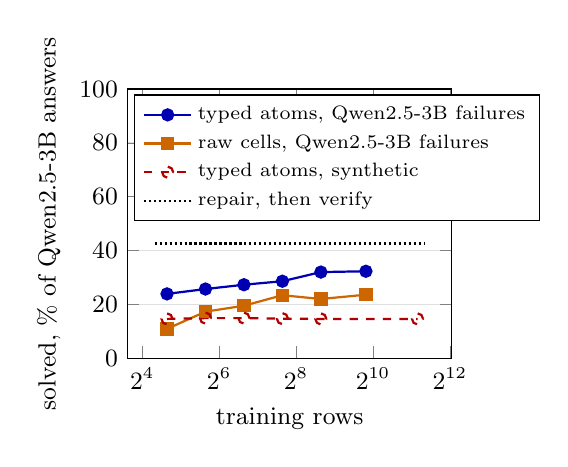
\begin{tikzpicture}
\begin{axis}[width=0.47\linewidth, height=5.0cm, xmode=log, log basis x=2, xlabel={training rows}, ylabel={solved, \% of Qwen2.5-3B answers},
  ymin=0, ymax=100, ymajorgrids, grid style={gray!25}, legend style={font=\scriptsize, at={(0.02,0.98)}, anchor=north west}, legend cell align=left,
  tick label style={font=\small}, label style={font=\small}]
\addplot[blue!70!black, mark=*, thick] coordinates {(25,23.9) (50,25.7) (100,27.3) (200,28.6) (400,32.0) (900,32.3)};
\addlegendentry{typed atoms, Qwen2.5-3B failures}
\addplot[orange!80!black, mark=square*, thick] coordinates {(25,10.9) (50,17.3) (100,19.5) (200,23.4) (400,22.0) (900,23.6)};
\addlegendentry{raw cells, Qwen2.5-3B failures}
\addplot[red!70!black, dashed, mark=o, thick] coordinates {(25,14.6) (50,14.9) (100,14.9) (200,14.7) (400,14.6) (2282,14.6)};
\addlegendentry{typed atoms, synthetic}
\addplot[black, densely dotted, thick, domain=20:2600, samples=2] {42.6};
\addlegendentry{repair, then verify}
\end{axis}
\end{tikzpicture}
\hfill
  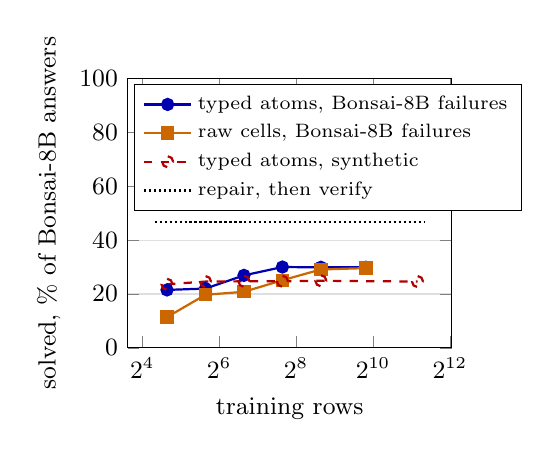
\begin{tikzpicture}
\begin{axis}[width=0.47\linewidth, height=5.0cm, xmode=log, log basis x=2, xlabel={training rows}, ylabel={solved, \% of Bonsai-8B answers},
  ymin=0, ymax=100, ymajorgrids, grid style={gray!25}, legend style={font=\scriptsize, at={(0.02,0.98)}, anchor=north west}, legend cell align=left,
  tick label style={font=\small}, label style={font=\small}]
\addplot[blue!70!black, mark=*, thick] coordinates {(25,21.5) (50,22.0) (100,26.9) (200,30.0) (400,29.9) (900,29.9)};
\addlegendentry{typed atoms, Bonsai-8B failures}
\addplot[orange!80!black, mark=square*, thick] coordinates {(25,11.4) (50,19.7) (100,20.8) (200,25.1) (400,29.1) (900,29.6)};
\addlegendentry{raw cells, Bonsai-8B failures}
\addplot[red!70!black, dashed, mark=o, thick] coordinates {(25,23.6) (50,24.6) (100,24.7) (200,24.7) (400,24.9) (2282,24.6)};
\addlegendentry{typed atoms, synthetic}
\addplot[black, densely dotted, thick, domain=20:2600, samples=2] {46.6};
\addlegendentry{repair, then verify}
\end{axis}
\end{tikzpicture}

  \caption{Learning curves, mean over five seeds: share of test answers solved against training rows, for gates trained on Qwen2.5-3B's failures and tested on its answers (left) and on Bonsai-8B's failures and answers (right). Dashed lines use synthetic defects; the dotted line is repair-then-verify.}
  \label{fig:curves}
\end{figure}

Table~\ref{tab:policies} and Figure~\ref{fig:curves} give the results.

\paragraph{The commit decision belongs to the verifier.} Repair-then-verify solves every answer any menu action can fix, 63 of 148 for Qwen2.5-3B and 69 for Bonsai-8B, and commits nothing broken. The published \texttt{dual\_repair} flow solves 62 and 69 and commits a broken grid on 86 and 79, because it never rejects. Verification costs about 1.8 repair calls and 2.7 verifier calls per item, milliseconds at these sizes.

\paragraph{A pre-repair gate cannot tell which answers the repair will fix.} The typed gate trained on all 900 of Qwen's train rows solves 48 of its test answers. It rejects 15 answers the repair would have fixed and commits a broken grid on 24 that no operator can fix; the Bonsai-8B gate on its own proposer is similar (45 solved, 20 unsafe). Both have far fewer unsafe commits than the published flow (G3q: \testGthreeq; G3: \testGthree). A post-hoc check asks whether a weak network or missing information is to blame: logistic regression and gradient-boosted trees fit on the same rows solve 34 to 47 of Qwen's answers with 19 to 32 unsafe, and 35 to 52 of Bonsai-8B's with 16 to 26 unsafe, separating fixable from unfixable answers with an AUC between 0.72 and 0.84. The limit is the information available before repair, not the tiny network. Put after the gate, the verifier removes every unsafe commit and keeps the gate's savings: 48 solved, none unsafe, about one call per item. That trade, fewer calls for fewer solved items, is the gate's only role here, and it pays only where repair or verification is expensive.

\paragraph{Declared atoms make a gate learnable from fewer rows.} For both proposers the typed gate learns faster than one on raw cells. At 25 rows it solves 24\% of Qwen's answers against 11\%, and 21\% of Bonsai-8B's against 11\% (seed means). For Qwen the gap persists to full size: 32\% against 24\% on average, and 48 against 37 solved for the seed-majority gates (G2q: \testGtwoq). For Bonsai-8B the two meet by 400 rows and do not differ at full size (G2: \testGtwo). This is the data-efficiency effect the April paper hypothesised. Its size depends on the proposer's failures, and neither representation approaches repair-then-verify.

\paragraph{Synthetic defects do not stand in for real failures.} A typed gate trained on synthetic defects reaches 98\% validation accuracy on synthetic defects. On Qwen's answers it then solves 21 and commits 66 broken grids, against 48 and 24 for the gate trained on Qwen's failures (G1q: \testGoneq). On Bonsai-8B's answers it commits 58 against 20; there the difference in solved items is not significant (G1: \testGone). A curriculum must come from real failures.

\paragraph{Transfer across proposers.} Table~\ref{tab:cross} crosses training source with test proposer. Bonsai-27B fails differently from both: its answers rarely have touching tents (14 of 148) but move trees in 92; one passes as written and 66 are fixable. A gate trained on one proposer's failures transfers partly to another's. Qwen's gate on Bonsai-8B's answers solves 43 with 22 unsafe, against 45 and 20 for Bonsai-8B's own gate, and still commits far fewer broken grids than the published flow (G4q: \testGfourq). Bonsai-8B's gate on Qwen's answers solves 38 against 48 for Qwen's own. On Bonsai-27B both commit 32 or more broken grids (G4: \testGfour). Repair-then-verify is complete and safe on all three proposers, which is one more reason to keep the verifier as the commit gate.

\begin{table}[t]
  \centering
  \small
  \begin{tabular}{lrrrrrr}
\toprule
Typed gate trained on & \multicolumn{2}{c}{Qwen2.5-3B answers} & \multicolumn{2}{c}{Bonsai-8B answers} & \multicolumn{2}{c}{Bonsai-27B answers} \\
\cmidrule(lr){2-3} \cmidrule(lr){4-5} \cmidrule(lr){6-7}
 & Solved & Unsafe & Solved & Unsafe & Solved & Unsafe \\
\midrule
Qwen2.5-3B failures & 48 & 24 & 43 & 22 & 54 & 39 \\
Bonsai-8B failures & 38 & 23 & 45 & 20 & 38 & 32 \\
Synthetic defects & 21 & 66 & 37 & 58 & 28 & 75 \\
Repair, then verify & 63 & 0 & 69 & 0 & 66 & 0 \\
\bottomrule
\end{tabular}

  \caption{Typed gates by training source (rows) and test proposer (columns), seed-majority actions on 148 greedy test answers each.}
  \label{tab:cross}
\end{table}

\section{A repair TRM trained on a MeTTa-framed corpus}
\label{sec:repair}

The gates of Section~\ref{sec:training} only choose among the skill's repair operators. This section trains a TRM that writes the repair itself and asks whether framing its training corpus with the MeTTa package helps. The design and four tests were registered before any repair model was built. Two further tests were registered after the validation runs and before any test prediction was read. A confirmation on fresh data was registered after the first test results.

\subsection{Setup}

\paragraph{Task.} Given a puzzle and a broken answer, the network outputs a tent or no tent for every non-tree cell; trees are copied from the puzzle and the decoded grid is scored by the verifier. The training target is the valid solution nearest the broken answer. Most puzzles have one solution (461 of the 506 study puzzles), and real broken answers sit a median of 6 cells from the nearest one, so the task is close to solving the puzzle with a noisy hint.

\paragraph{Corpus.} 4{,}528 real broken answers from Qwen2.5-3B and Bonsai-8B on 982 training puzzles (the original 300 plus 682 new ones, disjoint by hash from every other pool), with the 232 validation answers for selection. The test sets are those of Section~\ref{sec:training}.

\paragraph{Framings.} Both arms see the same rows, targets, network, and training budget; only the per-cell input differs. The \emph{raw} corpus gives each cell 8 channels: the candidate's symbol, whether the puzzle has a tree there, whether the cell is inside the grid, and the row and column tent targets. The \emph{atoms} corpus adds the 8 cell atoms a second MeTTa package declares, each a public rule localised to the cell it constrains:
\begin{itemize}[leftmargin=*]
  \item eligible: the cell is orthogonally next to a puzzle tree;
  \item row and column deficit: how many tents the cell's row or column still needs;
  \item row and column slack: eligible cells minus the target, per row or column;
  \item touching tent, unmatched tent, and tree mismatch.
\end{itemize}
The atoms are deterministic functions of the raw channels, so any gain is in what the network learns from the corpus, not in new information.

\paragraph{Model.} A TRM-style recursive network over the cells of a padded 6$\times$6 grid: one shared 2-layer transformer block (width 64, 4 heads) updates a latent state three times and then the answer state, for three cycles, and a per-cell logit is read from the answer (about 69{,}000 parameters). It is trained with binary cross-entropy and AdamW on a cosine schedule over 80 epochs; the learning rate (1e-3 or 3e-4) and the checkpoint (epoch 20, 40, or 80) are chosen on validation, and both arms chose 1e-3 at epoch 80. Five seeds are trained per arm, and the registered tests use the per-cell majority over them.

\subsection{Results}

\begin{table}[t]
  \centering
  \small
  \begin{tabular}{lrrr}
\toprule
Policy & Qwen2.5-3B & Bonsai-8B & Bonsai-27B \\
\midrule
Skill operators, then verify & 63 & 69 & 66 \\
Repair TRM, raw corpus & 73 & 71 & 73 \\
Repair TRM, MeTTa-atoms corpus & 78 & 81 & 77 \\
Operators, then raw TRM, then verify & 90 & 86 & 86 \\
Operators, then atoms TRM, then verify & 93 & 94 & 93 \\
CSP solver & 148 & 148 & 148 \\
\midrule
Single raw TRMs (5 seeds), range & 60--67 & 60--67 & 62--67 \\
Single atoms TRMs (5 seeds), range & 68--84 & 72--85 & 69--83 \\
\bottomrule
\end{tabular}

  \caption{Answers solved by the repair TRM and by the skill, of 148 greedy test answers from each proposer (columns). TRM rows are per-cell majorities over five seeds; the last two rows give the range over the five single models.}
  \label{tab:repair}
\end{table}

\begin{figure}[t]
  \centering
  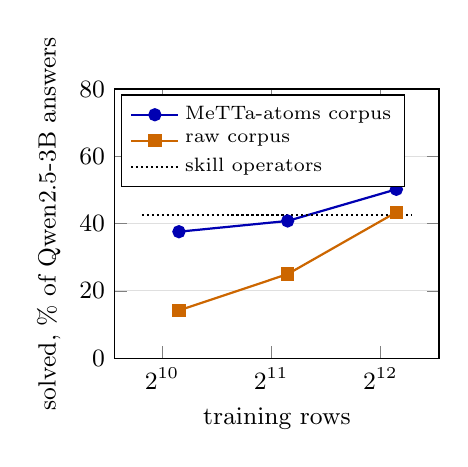
\begin{tikzpicture}
\begin{axis}[width=0.47\linewidth, height=5.0cm, xmode=log, log basis x=2, xlabel={training rows}, ylabel={solved, \% of Qwen2.5-3B answers},
  ymin=0, ymax=80, ymajorgrids, grid style={gray!25}, legend style={font=\scriptsize, at={(0.02,0.98)}, anchor=north west}, legend cell align=left,
  tick label style={font=\small}, label style={font=\small}]
\addplot[blue!70!black, mark=*, thick] coordinates {(1139,37.6) (2271,40.8) (4528,50.2)};
\addlegendentry{MeTTa-atoms corpus}
\addplot[orange!80!black, mark=square*, thick] coordinates {(1139,14.2) (2271,25.0) (4528,43.4)};
\addlegendentry{raw corpus}
\addplot[black, densely dotted, thick, domain=900:5000, samples=2] {42.6};
\addlegendentry{skill operators}
\end{axis}
\end{tikzpicture}
\hfill
  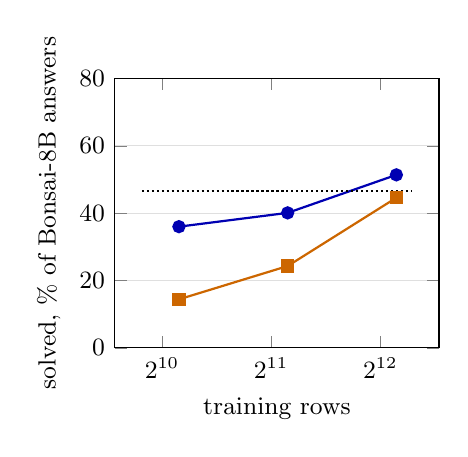
\begin{tikzpicture}
\begin{axis}[width=0.47\linewidth, height=5.0cm, xmode=log, log basis x=2, xlabel={training rows}, ylabel={solved, \% of Bonsai-8B answers},
  ymin=0, ymax=80, ymajorgrids, grid style={gray!25}, 
  tick label style={font=\small}, label style={font=\small}]
\addplot[blue!70!black, mark=*, thick] coordinates {(1139,36.0) (2271,40.1) (4528,51.4)};
\addplot[orange!80!black, mark=square*, thick] coordinates {(1139,14.4) (2271,24.3) (4528,44.6)};
\addplot[black, densely dotted, thick, domain=900:5000, samples=2] {46.6};
\end{axis}
\end{tikzpicture}

  \caption{Repair TRM learning curves, mean over seeds (three at a quarter and half of the training puzzles, five with all): share of test answers solved against training rows, on Qwen2.5-3B's answers (left) and Bonsai-8B's (right). The dotted line is the skill's own operators.}
  \label{fig:repair-curves}
\end{figure}

Table~\ref{tab:repair} and Figure~\ref{fig:repair-curves} give the results.

\paragraph{A repair TRM beats the skill's operators.} On Qwen2.5-3B's answers the atoms TRM alone solves 78 and the raw TRM 73, against 63 for the operators with verification. Placed after the operators in the repair-then-verify pipeline, the atoms TRM brings the skill from 63 to 93 solved answers with no broken commit (P3: \testPthree). The gains on Bonsai-8B's answers (69 to 94) and Bonsai-27B's (66 to 93) are similar.

\paragraph{With the full corpus, the framings do not separate as ensembles.} The five-seed majorities solve 78 against 73 on Qwen's answers (P1: \testPone) and 81 against 71 on Bonsai-8B's (P2: \testPtwo); inside the pipeline the atoms TRM leads 93 to 90 (P4: \testPfour).

\paragraph{With less data, the MeTTa framing matters a great deal.} Trained on a quarter of the puzzles, the atoms TRM solves 57 of Qwen's answers against 26 for raw (P5: \testPfive). On half, it solves 62 against 39 (P6: \testPsix). In seed means the atoms TRM solves 38\%, 41\%, and 50\% of Qwen's answers with a quarter, half, and all of the corpus; the raw TRM solves 14\%, 25\%, and 43\%. A quarter of the framed corpus buys about what the full raw corpus buys.

\paragraph{Single models and robustness.} At full size each of the five registered atoms models beat each of the five raw models on all three test sets (68 to 84 against 60 to 67 on Qwen's answers), and majority voting narrowed the gap because it helped raw more. Because this was noticed on the test sets, it was checked on a fresh pool of 141 puzzles with five new seeds per arm. Single atoms models solved 9.2 more of Qwen's answers than single raw models on average (\testCone, C1) and 10.0 more of Bonsai-8B's (\testCtwo, C2); the separation was no longer complete, since one atoms model scored below the best raw one on Qwen's answers. The new seeds overlap on the original test sets too (on Qwen's answers atoms 68--87 against raw 56--70), with the framed models ahead by 9 to 13 answers on average across the three proposers. The fresh five-model ensembles solve 68 against 60 and 71 against 61, where the skill's operators solve 62 and 68. The framing also makes training less fragile: at the lower learning rate the raw network reaches 9.5\% on validation and the atoms network 27.6\%.

\paragraph{Reading.} Here, unlike for the gates of Section~\ref{sec:training}, framing the corpus with declared atoms produces a benchmark benefit. It makes the repair network roughly three to four times as data-efficient and less sensitive to its learning rate, and a framed repair TRM adds 30 solved answers to the skill without a broken commit. The benefit shrinks as the raw network gets enough data to compute the same quantities itself, which is what one expects of features that are functions of the input. A symmetry-augmentation factor declared in the same package was registered as descriptive; its runs were not complete at this revision.

\section{Intellect-3 logic flow-policy replay}
\label{sec:flow}

A deterministic replay over 109 Campsite grids from an earlier Qwen3.5-27B run asked whether repair should be broad or narrow. The proposing arm, a logic skill with a task-representation memory, produced exactly correct grids on 33 of 109. Applying \texttt{c\_repair} whenever the count signature failed raised that to 74 of 109; repairing whenever either signature failed gave 73; multi-arm minimum-edit variants gave 72 (Table~\ref{tab:flow}). The narrow count repair was as good as anything broader.

\begin{table}[t]
  \centering
  \small
  \begin{tabular}{lrr}
    \toprule
    Policy & Exact, of 109 & Cell accuracy \\
    \midrule
    Proposing arm as written & 33 & 0.879 \\
    \texttt{c\_repair} if the count signature fails & 74 & 0.934 \\
    \texttt{dual\_repair} if any signature fails & 73 & 0.932 \\
    Multi-arm minimum-edit count repair & 72 & 0.932 \\
    Signature-first, then dual & 72 & 0.930 \\
    \bottomrule
  \end{tabular}
  \caption{Post-hoc replay of repair policies on 109 historical Campsite grids. No model was called; policies are applied to stored outputs.}
  \label{tab:flow}
\end{table}

Two cautions apply. The proposing arm routed on exact row-and-column constraint signatures matched against a support set of earlier rows; whether evaluated puzzles shared signatures with that support set was not audited, and the source data are not available to this revision, so the 33 of 109 is historical and not evidence of reasoning. And the replay scores exactness against stored answers; the repairs themselves read only the public counts, which we verified equal the answers' counts on the puzzles of Section~\ref{sec:training}.

\section{Verifier-state target definitions}
\label{sec:targets}

The April version reported three tables computed without any model. They define training targets; they are not results, because each reads post-repair state that is itself computed against the answer key.

\paragraph{Count-repair commit rule.} On a 122-row pack of count-signature repairs (86 train, 16 validation, 20 holdout), committing when the repaired grid is exact or its reward rose gives no false commits and no false rejects on any split. Committing whenever the repaired signatures pass commits every no-gain repair, because every repaired candidate passes the signatures by construction. Committing only exact grids rejects every partial improvement.

\paragraph{Nine-family separability matrix.} Over 148 before-and-after repair rows from nine families, the same post-repair rule separates commit from reject on every row; a family-specific symbolic check alone commits 66\% of the rows that should be rejected, all of them from the count-repair family; a pre-repair reward threshold commits 47\% of them and rejects 34\% of the rows that should commit. The four math rows are a negative control: no check produces a missing numeric answer.

\paragraph{Closure threshold.} A proposal-tier suite asks how complete a proposal must be before a symbolic circuit can finish it. Tool-call contracts, choice extraction, ASCII trees, and Campsite grids close from a partial proposal; math closes only from a full candidate.

Section~\ref{sec:training} replaces the reward-based rule with the deployable one: run the repair, then ask the public verifier.

\section{Environment-dependent compactification}
\label{sec:contracts}

Two suites test whether showing a model the validator's contract, and giving it one repair pass with the validator's feedback, helps it meet observable output contracts. The 50-row held-out suite covers word-count summaries, JSON schemas, ASCII trees, literal-count instructions, boolean and choice labels, and pipe-delimited records; the 30-row hard suite shifts toward numeric micro-math, logic labels, computed JSON, state sequences, and deeper trees. Each row has a frozen exact validator.

The April arms were named ``pure TRM'' and ``MeTTa runtime''. In the runner they show the same contract text and differ only in the system prompt: one says to parse, draft, and verify; the other lists a gate sequence. Neither calls a trained model or a MeTTa interpreter. We rename them for what they are and add the missing arm: the contract shown under the baseline's own system prompt. The April runner was executed unchanged with the re-obtained Qwen2.5-3B on CPU, with blind repair on both suites; the new arm uses the runner's own prompt builder and generation call.

\begin{table}[t]
  \centering
  \small
  \resizebox{\linewidth}{!}{\begin{tabular}{lrrrrrr}
\toprule
 & \multicolumn{3}{c}{Held-out, of 50} & \multicolumn{3}{c}{Hard, of 30} \\
\cmidrule(lr){2-4} \cmidrule(lr){5-7}
Arm & 3B, April & 3B, rerun & Bonsai-8B & 3B, April & 3B, rerun & Bonsai-8B \\
\midrule
Baseline & 23 & 24 & 22 & 12 & 9 & 8 \\
Contract, baseline system prompt & -- & 35 & 25 & -- & 11 & 9 \\
Contract, skill wording (April: pure TRM) & 27 & 28 & 24 & 11 & 11 & 10 \\
Contract, gate wording (April: MeTTa runtime) & 32 & 34 & 31 & 9 & 8 & 10 \\
Gate wording, then blind repair & -- & 36 & 32 & 12 & 13 & 12 \\
Gate wording, then validator-feedback repair & 37 & 39 & 32 & 13 & 13 & 14 \\
\bottomrule
\end{tabular}
}
  \caption{Exact successes on the output-contract suites, same rows across arms: the April Qwen2.5-3B run (blind repair was run only on the hard suite), this revision's CPU rerun of the April runner, and a second model, Bonsai-8B. Repair arms act only on rows the gate-wording arm got wrong.}
  \label{tab:contracts}
\end{table}

Table~\ref{tab:contracts}. The rerun reproduces the April run closely: the validator's verdict agrees with the April row on 48 to 50 of the 50 held-out rows per arm and on 27 to 30 of the 30 hard rows. The new arm separates what the April design confounded:
\begin{itemize}[leftmargin=*]
  \item \textbf{The contract is what helps.} Shown under the baseline's plain system prompt, the validator contract lifts the 3B from 24 to 35 exact (M1q: \testMoneq).
  \item \textbf{The MeTTa gate wording adds nothing.} With the contract shown in both, the gate-sequence system prompt scores 34 against 35 (M2q: \testMtwoq). The April ``MeTTa runtime'' lift over the baseline was the contract text.
  \item \textbf{Validator feedback is not clearly better than a blind second pass.} Feedback repair reaches 39 and blind repair 36 (M3q: \testMthreeq).
\end{itemize}
Bonsai-8B behaves differently on the first two points: the contract alone moves it little (M1: \testMone), the gate wording adds 6 rows without surviving correction (M2: \testMtwo), and the two repair passes tie (M3: \testMthree). On the hard suite no arm separates from the baseline at the 5\% level for either model, and no contract or repair arm of either model solves a state-sequence row. The claim that survives is narrower than April's and better measured: showing a small model the public contract helps where the failure is in the output's visible shape, by about a fifth of the held-out rows for the 3B; the MeTTa framing of that contract adds nothing measurable; and none of it supplies missing arithmetic or state tracking.

\section{Task-graph allocation}
\label{sec:allocation}

A 12-row diagnostic on Campsite asks whether the 3B model can be moved from solving to transcribing. Each row paraphrases a puzzle's public constraints; the answer grid is absent. A public solver closes every row once the constraints are machine-readable, so the only job left is extraction. A plain extraction prompt yields 0 of 12 solved after repair; a prompt framed by the constraint schema, 6; a prompt that names the four extraction gates, 9; a router of typed extraction scripts with no model, 12 (Figure~\ref{fig:campgate}). The residual model errors are transcription errors: a column count copied into a row count, a lost tree, a shifted coordinate. The April runner, executed unchanged with the re-obtained model on CPU, gives 0, 6, 8, and 12; the one difference is a single row in the gate-named arm. This is a 12-row, one-seed diagnostic without a control for prompt length, and we draw no interval from it.

\begin{figure}[t]
  \centering
  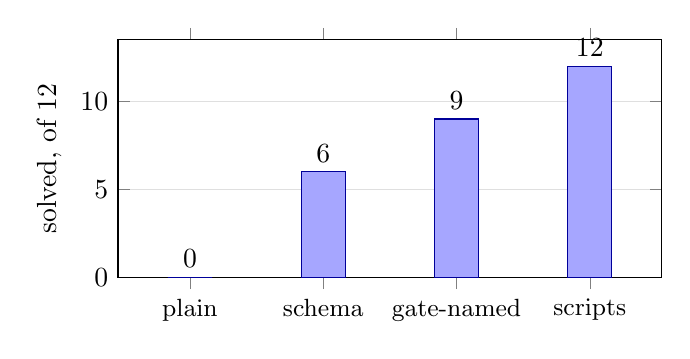
\begin{tikzpicture}
    \begin{axis}[ybar, bar width=16pt, width=0.7\linewidth, height=4.6cm, ymin=0, ymax=13.5, ylabel={solved, of 12},
      symbolic x coords={plain, schema, gate-named, scripts}, xtick=data,
      x tick label style={font=\small}, nodes near coords, enlarge x limits=0.18, ymajorgrids, grid style={gray!25}]
      \addplot[fill=blue!35, draw=blue!60!black] coordinates {(plain,0) (schema,6) (gate-named,9) (scripts,12)};
    \end{axis}
  \end{tikzpicture}
  \caption{Campsite constraint extraction from paraphrases, Qwen2.5-3B (April run), solved after a schema repair pass: a plain extraction prompt, a schema-framed prompt, a prompt naming the four extraction gates, and typed extraction scripts with no model.}
  \label{fig:campgate}
\end{figure}

The lesson is the one Section~\ref{sec:training} tests at scale: once a skill names its gates, stable gates move to scripts, closure moves to a solver or verifier, uncertain gates become training targets, and the language model is left to propose. On Campsite this allocation ends at the solver, which closes every puzzle in milliseconds; repair is never the cheapest path to a solved grid here, and we use the environment to study the curriculum and gate methodology, not to recommend repair for Campsite.

\section{Interpretation}
\label{sec:interpretation}

The evidence supports a staged skill design, with each stage owned by a different executor.
\begin{enumerate}[leftmargin=*]
  \item \textbf{Declare the state.} The MeTTa package names the verifier atoms, the operators and their preconditions, and the action menu. This is what makes failures typed, rows trainable, and evaluation automatic.
  \item \textbf{Narrow the action space by rule.} Where the operator follows from a visible label, a table chooses it; on the April curriculum this is the whole of the action-space lift.
  \item \textbf{Repair, then verify.} The commit decision is a call to the public verifier on the repaired output. On real near-misses this is the only policy that is both complete and safe, and it costs a few milliseconds per item at these sizes.
  \item \textbf{Train gates only where a decision is uncertain and expensive.} A tiny gate trained on the proposer's own near-misses can skip repairs that will not work. Typed atoms make it learnable from fewer rows, but it cannot see what the repair will do, so it trades solved items for saved calls, and it should sit in front of the verifier, not in place of it.
  \item \textbf{Train a repair TRM where the operators stop.} A recursive network that writes the repair fixes answers the declared operators cannot, and the verifier keeps it safe. This is where the MeTTa framing of the corpus pays most: the declared cell atoms let the network learn the repair from a fraction of the data.
  \item \textbf{Let the language model propose.} It writes the candidate and reads free text. No small model here made the commit decision well without leaked labels: the 3B's commit decisions were a constant, and the best honest arm, Bonsai-8B with clean retrieval, still committed 9 of the 22 no-gain repairs.
\end{enumerate}
The compactification claim of the April version survives in this narrower form: a small model becomes useful once the skill around it owns validation, repair, and commit. It does not survive as ``the LLM can shrink to a rudder'': on the rudder benchmark the model's share of the best arm was a constant, and on the output-contract suites the April model's lift came from seeing the contract, not from the MeTTa framing around it.

\section{Scope and limitations}
\label{sec:limits}

\begin{itemize}[leftmargin=*]
  \item \textbf{Size and independence.} The rudder benchmark has 88 rows from 44 problems; the Campsite tests have 148 puzzles, with 141 more for the repair TRM confirmation; the output-contract suites have 50 and 30 rows. Every model result is one seed with deterministic decoding. Trained gates and repair TRMs use five seeds, and registered tests use their per-item majority so that the unit is the puzzle.
  \item \textbf{Models and builds.} The April model, Qwen2.5-3B-Instruct at 4 bits, was re-obtained and runs on CPU with a different llama.cpp build from April's CUDA build. The replicated arms agree with the April rows on 84 to 88 of 88, except the leaky retrieval arm (73 of 88). Bonsai-8B and Bonsai-27B are 1-bit models. Real training rows come from two proposers.
  \item \textbf{Campsite is solvable.} A public CSP solver closes every puzzle here in milliseconds, so the environment measures the curriculum, gate, and repair-model methodology, not the best way to solve Campsite. The methodology is meant for environments without cheap closure.
  \item \textbf{The MeTTa ablation.} No experiment compares a MeTTa package with the same atoms written directly as JSON or Python. What the typed-versus-raw comparison shows is the value of declaring verifier-visible atoms, not of the language they are declared in.
  \item \textbf{Historical numbers.} The April 16--22 baseline and the 109-grid flow-policy replay are reported from their ledgers and were not re-measured; the replay's proposing arm was not audited for overlap with its support set.
  \item \textbf{Post-hoc analysis.} Two checks, the classifier comparisons in Section~\ref{sec:training} for each real curriculum, were added after the registered tests were computed. In Section~\ref{sec:repair} the low-data tests were registered after validation runs and the single-model confirmation after the first test results, on a fresh test pool with new seeds. None changes a registered result.
  \item \textbf{The repair TRM's limits.} It is trained and tested on the failures of the same two proposer families; the full-corpus ensemble comparison of the framings is not significant; and the symmetry factor declared in the same package had not finished.
\end{itemize}

\section{Conclusion}

Near-miss outputs are typed, repairable, and trainable, as the April version argued. What the measurements add is where each decision belongs. The repair operator follows from the failure label; the commit decision follows from the public verifier after repair; a tiny recursive gate trained on the proposer's own MeTTa-typed near-misses can save calls before repair, learns from fewer rows than one trained on raw cells, and cannot replace the verifier because the information it would need does not exist before the repair runs. A curriculum built from synthetic defects does not stand in for real failures. On output contracts, the April model gains from seeing the contract, and the MeTTa framing adds nothing measurable. Where the framing does pay is in training a TRM that writes the repair: declared cell atoms make it three to four times as data-efficient, and behind the verifier it adds 30 solved answers to the skill. The practical method is the one the April conclusion named, with the roles made precise: decompose the skill into declared gates, give each gate to the smallest reliable executor, verify before committing, and train only the gates that remain uncertain, on the failures of the model that will actually propose.

\bibliographystyle{plainnat}
\bibliography{references}

\appendix

\section{Corrections to the April version}
\label{app:corrections}

For readers of the April 29 report:
\begin{itemize}[leftmargin=*]
  \item ``TRM'' referred both to a task-representation memory and to tiny recursive models; Section~\ref{sec:baseline} separates them. No tiny recursive model had been trained on the curriculum; Section~\ref{sec:training} trains and tests one.
  \item The retrieval arm of the rudder benchmark selected examples using the eval row's own label. Its April reading (retrieved context improves commit decisions at 3B but hurts repair choice) and the May reading (9B and 27B reach 70 of 88 with retrieval) are withdrawn. Rerun with the April model and code on CPU, the arm scores 17 rather than 28, because its repair choice sits on near-tied tokens.
  \item The unseen-family split could not be answered by any model-decided arm, so the April ``unseen-family transfer'' numbers are withdrawn; with all actions listed, transfer is 1 of 18.
  \item The static-gate arm's 84 of 88 replicates exactly, with the same answer on every row; the model's share of it equals a policy that always commits. The May 88 of 88 restates the label.
  \item The ``pure TRM'' and ``MeTTa runtime'' arms of the output-contract suites differ only in system-prompt wording; they are renamed, and an arm separating contract from wording is added. With the April model the contract alone accounts for the lift.
  \item The post-repair verifier sweep, the nine-family matrix, and the closure suite are target definitions computed from answer-derived state, not results.
  \item Two state fields of the April curriculum (reward, and exact versus wrong-cell) are computed against the answer key; the rows carry no candidate content.
  \item The 33 of 109 starting point of the flow-policy replay comes from an arm whose support set was not audited for overlap with the evaluated puzzles.
  \item Figures with unreadable tick labels were replaced; tables now report counts with intervals or paired tests.
\end{itemize}
The retrieval leak, the unreachable split, and the failure of synthetic-defect gates on real proposals were first observed in a concurrent Morality Lab replication of this benchmark (the jev-qwen project, October 2026). This revision measures them independently, with its own registration, code, and models.

\section{Reproduction}
\label{app:repro}

The study is registered in \path{SPEC.md} in the directory \path{research/studies/2026-10-08-metta-curated-campsite-curriculum/}, with four dated addenda; the Qwen2.5-3B replication was registered in the third, before any Qwen call. The model file is \texttt{qwen2.5-3b-instruct-q4\_k\_m.gguf} from the Qwen/Qwen2.5-3B-Instruct-GGUF repository at revision \texttt{7dabda4d}, SHA-256 \texttt{626b4a66}\ldots\texttt{c62d}; \path{src/qwen_replicate.py} runs the April runners from git. The repair TRM study is registered in \path{SPEC-repair-trm.md} in the same directory, with three addenda; \path{src/repair_trm.py} trains it and \path{src/repair_report.py} computes its tests. Its \path{src/} directory holds the MeTTa package compiler, the Campsite layer (puzzles, verifier, and the skill's repair operators executed from the committed source), the proposal collector, the curriculum builder, the gate trainer, the rudder and output-contract reruns, and the report. Every result table in this paper is generated from \path{results/report.json} by \path{src/paper_tables.py}. Models run on CPU through a llama.cpp server with no GPU layers; the gates train on CPU in about ten minutes for all 270 configurations. The April artifacts cited in Sections~\ref{sec:rudder} to \ref{sec:allocation} are in the same repository \citep{hermesskills2026artifacts} under \path{research/generated} and \path{research/studies}.

\end{document}
